\subsection{\textit{Unified View of Parameter-Efficient Transfer Learning}}

\textit{Unified Parameter Transfer Learning} merupakan strategi dalam \textit{transfer learning} yang berupaya menggabungkan berbagai teknik adaptasi ke dalam satu kerangka kerja terpadu \parencite{uvpl}. Tujuan utamanya adalah untuk memaksimalkan efisiensi dan efektivitas saat mengadaptasi \textit{pre-trained model} untuk tugas-tugas baru.

Dalam \textit{transfer learning}, ide utamanya adalah mengambil model yang telah dilatih pada satu tugas dan menyesuaikannya untuk tugas yang berbeda. Namun, ada banyak cara untuk melakukan adaptasi ini, dan setiap metode memiliki kelebihan dan kekurangannya sendiri. Beberapa teknik mungkin fokus pada penambahan lapisan adaptasi, sementara yang lain mungkin memprioritaskan modifikasi parameter tertentu dalam model.

Alih-alih memilih satu teknik adaptasi dan berkomitmen padanya, pendekatan ini menggabungkan berbagai teknik untuk menciptakan solusi adaptasi yang lebih komprehensif. Dengan demikian, model yang diadaptasi dengan metode ini dapat memanfaatkan kelebihan dari berbagai teknik adaptasi, sambil menghindari atau meminimalkan kekurangan masing-masing teknik.

Misalnya, satu teknik adaptasi mungkin sangat efektif untuk tugas klasifikasi tetapi kurang optimal untuk tugas generasi teks. Dengan pendekatan terpadu, model dapat memanfaatkan teknik adaptasi yang paling sesuai untuk setiap tugas, memungkinkan kinerja yang lebih baik dan adaptasi yang lebih cepat.

Selain itu, dengan menggabungkan berbagai teknik, \textit{Unified View of Parameter-Efficient Transfer Learning} juga memungkinkan peneliti untuk bereksperimen dan menemukan kombinasi teknik yang paling efektif untuk tugas atau dataset tertentu. Ini memberikan fleksibilitas tambahan dan memungkinkan adaptasi yang lebih disesuaikan dengan kebutuhan spesifik.

\begin{figure}[ht]
    \centering
    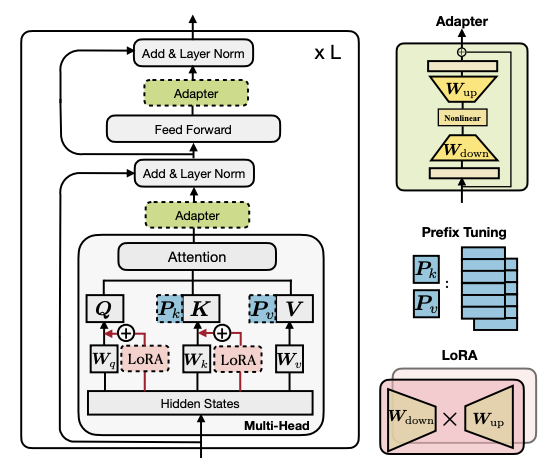
\includegraphics[width=0.8\textwidth]{chapter-2/uvpl.png}
    \caption{Arsitektur \textit{Unified View of Parameter-Efficient Transfer Learning} \parencite{uvpl}}
    \label{fig:uvpl}
\end{figure}

Dengan demikian, \textit{Unified View} ini menawarkan pendekatan adaptasi yang inovatif dan fleksibel, yang memungkinkan \textit{pre-trained model} untuk menyesuaikan diri dengan berbagai tugas dengan efisiensi dan efektivitas yang lebih tinggi.